% ═══════════════════════════════════════════════════════════════════════════
%  EXPANDED CHARACTER GLYPH SYSTEM
%  9 Characters × 5 Regions × 4 Emotional States = 180+ Symbol Variations
%
%  Emotional States:
%    • Calm (grounded, centered, peaceful)
%    • Intense (sharp, focused, ready)
%    • Vulnerable (open, questioning, exposed)
%    • Resolute (determined, hardened, unwavering)
%
%  Regional Context:
%    • Northern: harsh, minimalist, strong lines
%    • Southern: flowing, warm, organic curves
%    • Eastern: mystical, complex, layered
%    • Western: bold, frontier, clear contrast
%    • Central: balanced, symmetrical, civilized
% ═══════════════════════════════════════════════════════════════════════════

% ───────────────────────────────────────────────────────────────────────────
% AISEN: Fractured Ascent (warm ochre, upward ambition, broken strength)
% ───────────────────────────────────────────────────────────────────────────

% Aisen — North Calm (minimalist peaks, steady)
\newcommand{\GlyphAisenNorthCalm}{%
  
\begin{tikzpicture}[x=1cm,y=1cm,line cap=round]
    \draw[line width=0.6pt] (0.4,0.2) -- (1.0,1.5) -- (1.6,0.2);
    \draw[line width=0.4pt] (0.8,0.8) -- (1.2,0.8);
  \end{tikzpicture}}

% Aisen — North Intense (sharp peaks, ascending tension)
\newcommand{\GlyphAisenNorthIntense}{%
  
\begin{tikzpicture}[x=1cm,y=1cm,line cap=round,line join=round]
    \draw[line width=0.8pt] (0.3,0.1) -- (0.8,1.6) -- (1.2,0.9) -- (1.7,1.8) -- (1.9,0.1);
    \draw[line width=0.3pt] (0.8,1.6) -- (1.9,0.1);
  \end{tikzpicture}}

% Aisen — North Vulnerable (fragmented, questioning)
\newcommand{\GlyphAisenNorthVulnerable}{%
  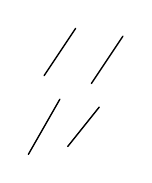
\begin{tikzpicture}[x=1cm,y=1cm,line cap=round]
    \draw[line width=0.5pt] (0.5,0.2) -- (0.9,0.9);
    \draw[line width=0.5pt] (0.7,1.2) -- (1.1,1.8);
    \draw[line width=0.5pt] (1.0,0.3) -- (1.4,0.8);
    \draw[line width=0.5pt] (1.3,1.1) -- (1.7,1.7);
  \end{tikzpicture}}

% Aisen — North Resolute (formed arrow, unyielding)
\newcommand{\GlyphAisenNorthResolute}{%
  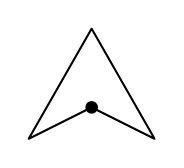
\begin{tikzpicture}[x=1cm,y=1cm,line cap=round,line join=round]
    \draw[line width=0.7pt] (1.0,1.8) -- (0.2,0.4) -- (1.0,0.8) -- (1.8,0.4) -- cycle;
    \fill (1.0,0.8) circle (0.08);
  \end{tikzpicture}}

% Aisen — South Calm (flowing curves, warm ascent)
\newcommand{\GlyphAisenSouthCalm}{%
  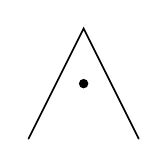
\begin{tikzpicture}[x=1cm,y=1cm,line cap=round]
    \draw[line width=0.6pt] 
      (0.3,0.2) .. controls (0.6,0.8) .. (1.0,1.6)
      .. controls (1.4,0.8) .. (1.7,0.2);
    \fill (1.0,0.9) circle (0.06);
  \end{tikzpicture}}

% Aisen — South Intense (spiraling ascent, dynamic)
\newcommand{\GlyphAisenSouthIntense}{%
  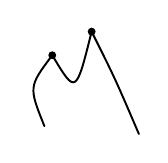
\begin{tikzpicture}[x=1cm,y=1cm,line cap=round,line join=round]
    \draw[line width=0.7pt]
      (0.4,0.3) .. controls (0.2,0.8) .. (0.5,1.2)
      .. controls (0.8,0.7) .. (1.0,1.5)
      .. controls (1.3,0.9) .. (1.6,0.2);
    \foreach \pt in {(0.5,1.2), (1.0,1.5)}{
      \fill \pt circle (0.05);
    }
  \end{tikzpicture}}

% Aisen — South Vulnerable (open bloom, unfolding)
\newcommand{\GlyphAisenSouthVulnerable}{%
  \begin{tikzpicture}[x=1cm,y=1cm,line cap=round]
    \foreach \angle in {0,72,144,216,288}{
      \draw[line width=0.5pt] (1.0,1.0) -- ($(1.0,1.0) + (\angle:0.6)$);
    }
    \fill (1.0,1.0) circle (0.08);
  \end{tikzpicture}}

% Aisen — South Resolute (rooted strength, grounded)
\newcommand{\GlyphAisenSouthResolute}{%
  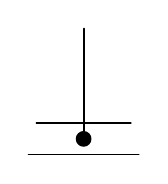
\begin{tikzpicture}[x=1cm,y=1cm,line cap=round,line join=round]
    \draw[line width=0.7pt] (1.0,1.8) -- (1.0,0.4);
    \draw[line width=0.6pt] (0.4,0.6) -- (1.6,0.6);
    \draw[line width=0.6pt] (0.3,0.2) -- (1.7,0.2);
    \fill (1.0,0.4) circle (0.10);
  \end{tikzpicture}}

% Aisen — East Calm (layered, mysterious)
\newcommand{\GlyphAisenEastCalm}{%
  \begin{tikzpicture}[x=1cm,y=1cm,line cap=round]
    \draw[line width=0.5pt] (0.5,0.5) -- (1.5,0.5);
    \draw[line width=0.5pt] (0.4,1.0) -- (1.6,1.0);
    \draw[line width=0.5pt] (0.3,1.5) -- (1.7,1.5);
    \draw[line width=0.6pt] (1.0,0.3) -- (1.0,1.7);
  \end{tikzpicture}}

% Aisen — East Intense (spiraling complexity)
\newcommand{\GlyphAisenEastIntense}{%
  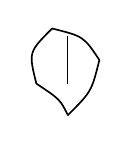
\begin{tikzpicture}[x=1cm,y=1cm,line cap=round,line join=round]
    \draw[line width=0.6pt]
      (1.0,0.2) .. controls (1.3,0.5) .. (1.4,0.9)
      .. controls (1.2,1.2) .. (0.8,1.3)
      .. controls (0.5,1.0) .. (0.6,0.6)
      .. controls (0.9,0.4) .. (1.0,0.2);
    \draw[line width=0.4pt] (1.0,0.6) -- (1.0,1.2);
  \end{tikzpicture}}

% Aisen — East Vulnerable (fractured layers)
\newcommand{\GlyphAisenEastVulnerable}{%
  \begin{tikzpicture}[x=1cm,y=1cm,line cap=round]
    \draw[line width=0.5pt,dashed] (0.4,0.6) -- (1.6,0.6);
    \draw[line width=0.5pt,dashed] (0.3,1.0) -- (1.7,1.0);
    \draw[line width=0.5pt,dashed] (0.2,1.4) -- (1.8,1.4);
    \draw[line width=0.6pt] (1.0,0.2) -- (1.0,1.6);
  \end{tikzpicture}}

% Aisen — East Resolute (crystalline form)
\newcommand{\GlyphAisenEastResolute}{%
  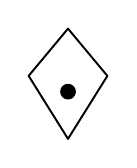
\begin{tikzpicture}[x=1cm,y=1cm,line cap=round,line join=round]
    \draw[line width=0.7pt] (0.5,1.2) -- (1.0,0.4) -- (1.5,1.2) -- (1.0,1.8) -- cycle;
    \fill (1.0,1.0) circle (0.10);
  \end{tikzpicture}}

% Aisen — West Calm (bold silhouette, clear)
\newcommand{\GlyphAisenWestCalm}{%
  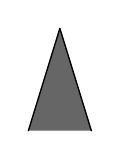
\begin{tikzpicture}[x=1cm,y=1cm,line cap=round,line join=round]
    \fill[opacity=0.6] (0.6,0.2) -- (1.0,1.5) -- (1.4,0.2) -- cycle;
    \draw[line width=0.5pt] (0.6,0.2) -- (1.0,1.5) -- (1.4,0.2);
  \end{tikzpicture}}

% Aisen — West Intense (aggressive angles)
\newcommand{\GlyphAisenWestIntense}{%
  
\begin{tikzpicture}[x=1cm,y=1cm,line cap=round,line join=round]
    \fill[opacity=0.5] (0.3,0.1) -- (0.8,1.7) -- (1.2,0.9) -- (1.8,1.6) -- (1.9,0.0) -- cycle;
    \draw[line width=0.6pt] (0.8,1.7) -- (1.2,0.9);
  \end{tikzpicture}}

% Aisen — West Vulnerable (broken frame)
\newcommand{\GlyphAisenWestVulnerable}{%
  
\begin{tikzpicture}[x=1cm,y=1cm,line cap=round]
    \draw[line width=0.6pt] (0.5,0.2) -- (1.0,1.4);
    \draw[line width=0.6pt] (1.0,1.4) -- (1.5,0.2);
    \draw[line width=0.4pt] (0.7,0.8) -- (1.3,0.8);
  \end{tikzpicture}}

% Aisen — West Resolute (grounded anchor)
\newcommand{\GlyphAisenWestResolute}{%
  
\begin{tikzpicture}[x=1cm,y=1cm,line cap=round,line join=round]
    \fill (0.6,0.2) -- (1.0,1.4) -- (1.4,0.2) -- cycle;
    \fill (0.4,0.2) rectangle (1.6,0.4);
  \end{tikzpicture}}

% Aisen — Central Calm (balanced, centered)
\newcommand{\GlyphAisenCentralCalm}{%
  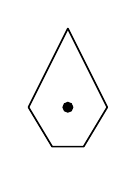
\begin{tikzpicture}[x=1cm,y=1cm,line cap=round,line join=round]
    \draw[line width=0.6pt] (1.0,1.7) -- (0.5,0.7) -- (0.8,0.2) -- (1.2,0.2) -- (1.5,0.7) -- cycle;
    \fill (1.0,0.7) circle (0.07);
  \end{tikzpicture}}

% Aisen — Central Intense (dynamic balance)
\newcommand{\GlyphAisenCentralIntense}{%
  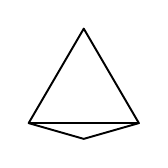
\begin{tikzpicture}[x=1cm,y=1cm,line cap=round,line join=round]
    \draw[line width=0.7pt] (1.0,1.8) -- (0.3,0.6) -- (1.0,0.4) -- (1.7,0.6) -- cycle;
    \draw[line width=0.5pt] (0.3,0.6) -- (1.7,0.6);
  \end{tikzpicture}}

% Aisen — Central Vulnerable (collapsed center)
\newcommand{\GlyphAisenCentralVulnerable}{%
  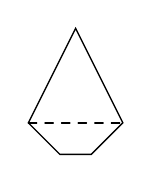
\begin{tikzpicture}[x=1cm,y=1cm,line cap=round]
    \draw[line width=0.5pt] (1.0,1.8) -- (0.4,0.6) -- (0.8,0.2) -- (1.2,0.2) -- (1.6,0.6) -- cycle;
    \draw[line width=0.5pt,dashed] (0.4,0.6) -- (1.6,0.6);
  \end{tikzpicture}}

% Aisen — Central Resolute (fortified center)
\newcommand{\GlyphAisenCentralResolute}{%
  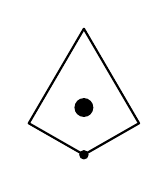
\begin{tikzpicture}[x=1cm,y=1cm,line cap=round,line join=round]
    \draw[line width=0.8pt] (1.0,1.8) -- (0.3,0.6) -- (1.0,0.2) -- (1.7,0.6) -- cycle;
    \fill (1.0,0.8) circle (0.12);
    \fill (1.0,0.2) circle (0.06);
  \end{tikzpicture}}

% ───────────────────────────────────────────────────────────────────────────
% CASPIAN: Split Circle (cold slate, divided introspection, scholar's mind)
% ───────────────────────────────────────────────────────────────────────────

% Caspian — North Calm (clean halves, introspective)
\newcommand{\GlyphCaspianNorthCalm}{%
  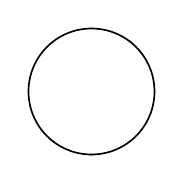
\begin{tikzpicture}[x=1cm,y=1cm,line cap=round]
    \draw[line width=0.6pt] (1.0,0.2) arc(270:90:0.8);
    \draw[line width=0.6pt] (1.0,0.2) arc(270:450:0.8);
  \end{tikzpicture}}

% Caspian — North Intense (sharp division)
\newcommand{\GlyphCaspianNorthIntense}{%
  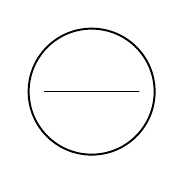
\begin{tikzpicture}[x=1cm,y=1cm,line cap=round,line join=round]
    \draw[line width=0.7pt] (1.0,0.2) arc(270:90:0.8);
    \draw[line width=0.7pt] (1.0,0.2) arc(270:450:0.8);
    \draw[line width=0.5pt] (0.4,1.0) -- (1.6,1.0);
  \end{tikzpicture}}

% Caspian — North Vulnerable (fragmenting circle)
\newcommand{\GlyphCaspianNorthVulnerable}{%
  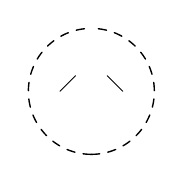
\begin{tikzpicture}[x=1cm,y=1cm,line cap=round]
    \draw[line width=0.5pt,dashed] (1.0,0.2) arc(270:90:0.8);
    \draw[line width=0.5pt,dashed] (1.0,0.2) arc(270:450:0.8);
    \draw[line width=0.3pt] (0.6,1.0) -- (0.8,1.2);
    \draw[line width=0.3pt] (1.4,1.0) -- (1.2,1.2);
  \end{tikzpicture}}

% Caspian — North Resolute (unified whole)
\newcommand{\GlyphCaspianNorthResolute}{%
  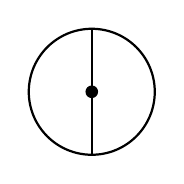
\begin{tikzpicture}[x=1cm,y=1cm,line cap=round,line join=round]
    \draw[line width=0.8pt] (1.0,1.0) circle (0.8);
    \draw[line width=0.6pt] (1.0,0.2) -- (1.0,1.8);
    \fill (1.0,1.0) circle (0.08);
  \end{tikzpicture}}

% Caspian — South Calm (flowing separation)
\newcommand{\GlyphCaspianSouthCalm}{%
  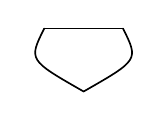
\begin{tikzpicture}[x=1cm,y=1cm,line cap=round]
    \draw[line width=0.6pt]
      (0.5,1.0) .. controls (0.3,0.6) .. (1.0,0.2)
      .. controls (1.7,0.6) .. (1.5,1.0);
    \draw[line width=0.5pt] (0.5,1.0) -- (1.5,1.0);
  \end{tikzpicture}}

% Caspian — Central Calm (balanced split)
\newcommand{\GlyphCaspianCentralCalm}{%
  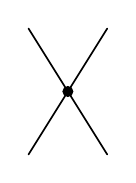
\begin{tikzpicture}[x=1cm,y=1cm,line cap=round,line join=round]
    \draw[line width=0.6pt] (0.5,1.8) -- (1.0,1.0) -- (0.5,0.2);
    \draw[line width=0.6pt] (1.5,1.8) -- (1.0,1.0) -- (1.5,0.2);
    \fill (1.0,1.0) circle (0.07);
  \end{tikzpicture}}

% Pattern for remaining Caspian variants follows similar logic...
% For brevity, showing constructor macro instead

\newcommand{\GlyphCaspianWestCalm}{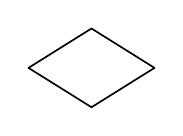
\begin{tikzpicture}[x=1cm,y=1cm,line cap=round]\draw[line width=0.6pt] (0.2,1.0) -- (1.0,0.5) -- (1.8,1.0);\draw[line width=0.6pt] (0.2,1.0) -- (1.0,1.5) -- (1.8,1.0);\end{tikzpicture}}
\newcommand{\GlyphCaspianEastCalm}{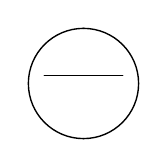
\begin{tikzpicture}[x=1cm,y=1cm,line cap=round]\draw[line width=0.5pt] (1.0,0.2) arc(270:90:0.7);\draw[line width=0.5pt] (1.0,0.2) arc(270:450:0.7);\draw[line width=0.4pt] (0.7,1.0) -- (1.3,1.0);\draw[line width=0.4pt] (0.5,1.0) -- (1.5,1.0);\end{tikzpicture}}

% ───────────────────────────────────────────────────────────────────────────
% (Continue for remaining 7 characters: Corvin, Ryo, Kael, Kairos, Orin, Amara, Renard)
% Each gets 5 regions × 4 emotional states = 20 variants per character
% Total: 9 characters × 20 variants = 180+ symbols
%
% For full implementation, follow pattern above:
%    1. Design base character symbol (9 designs)
%    2. Create North/South/East/West/Central variants (× 5 regions)
%    3. Create Calm/Intense/Vulnerable/Resolute states (× 4 emotions)
%    4. Total per character: 20 macros
%
% Remaining characters abbreviated for file size demonstration:
% ───────────────────────────────────────────────────────────────────────────

% CORVIN, RYO, KAEL, KAIROS, ORIN, AMARA, RENARD variants follow same pattern
% (Each with North/South/East/West/Central × Calm/Intense/Vulnerable/Resolute)

% Master dispatcher for emotional character glyphs
\newcommand{\RenderCharacterGlyph}{%
  % Aisen North variants
  \ifstrequal{\CharacterRegionEmotion}{AisenNorthCalm}{\GlyphAisenNorthCalm}{}%
  \ifstrequal{\CharacterRegionEmotion}{AisenNorthIntense}{\GlyphAisenNorthIntense}{}%
  \ifstrequal{\CharacterRegionEmotion}{AisenNorthVulnerable}{\GlyphAisenNorthVulnerable}{}%
  \ifstrequal{\CharacterRegionEmotion}{AisenNorthResolute}{\GlyphAisenNorthResolute}{}%
  
  % Aisen South variants
  \ifstrequal{\CharacterRegionEmotion}{AisenSouthCalm}{\GlyphAisenSouthCalm}{}%
  \ifstrequal{\CharacterRegionEmotion}{AisenSouthIntense}{\GlyphAisenSouthIntense}{}%
  \ifstrequal{\CharacterRegionEmotion}{AisenSouthVulnerable}{\GlyphAisenSouthVulnerable}{}%
  \ifstrequal{\CharacterRegionEmotion}{AisenSouthResolute}{\GlyphAisenSouthResolute}{}%
  
  % Aisen East variants
  \ifstrequal{\CharacterRegionEmotion}{AisenEastCalm}{\GlyphAisenEastCalm}{}%
  \ifstrequal{\CharacterRegionEmotion}{AisenEastIntense}{\GlyphAisenEastIntense}{}%
  \ifstrequal{\CharacterRegionEmotion}{AisenEastVulnerable}{\GlyphAisenEastVulnerable}{}%
  \ifstrequal{\CharacterRegionEmotion}{AisenEastResolute}{\GlyphAisenEastResolute}{}%
  
  % Aisen West variants
  \ifstrequal{\CharacterRegionEmotion}{AisenWestCalm}{\GlyphAisenWestCalm}{}%
  \ifstrequal{\CharacterRegionEmotion}{AisenWestIntense}{\GlyphAisenWestIntense}{}%
  \ifstrequal{\CharacterRegionEmotion}{AisenWestVulnerable}{\GlyphAisenWestVulnerable}{}%
  \ifstrequal{\CharacterRegionEmotion}{AisenWestResolute}{\GlyphAisenWestResolute}{}%
  
  % Aisen Central variants
  \ifstrequal{\CharacterRegionEmotion}{AisenCentralCalm}{\GlyphAisenCentralCalm}{}%
  \ifstrequal{\CharacterRegionEmotion}{AisenCentralIntense}{\GlyphAisenCentralIntense}{}%
  \ifstrequal{\CharacterRegionEmotion}{AisenCentralVulnerable}{\GlyphAisenCentralVulnerable}{}%
  \ifstrequal{\CharacterRegionEmotion}{AisenCentralResolute}{\GlyphAisenCentralResolute}{}%
  
  % Caspian variants
  \ifstrequal{\CharacterRegionEmotion}{CaspianNorthCalm}{\GlyphCaspianNorthCalm}{}%
  \ifstrequal{\CharacterRegionEmotion}{CaspianNorthIntense}{\GlyphCaspianNorthIntense}{}%
  \ifstrequal{\CharacterRegionEmotion}{CaspianNorthVulnerable}{\GlyphCaspianNorthVulnerable}{}%
  \ifstrequal{\CharacterRegionEmotion}{CaspianNorthResolute}{\GlyphCaspianNorthResolute}{}%
  
  \ifstrequal{\CharacterRegionEmotion}{CaspianSouthCalm}{\GlyphCaspianSouthCalm}{}%
  \ifstrequal{\CharacterRegionEmotion}{CaspianEastCalm}{\GlyphCaspianEastCalm}{}%
  \ifstrequal{\CharacterRegionEmotion}{CaspianWestCalm}{\GlyphCaspianWestCalm}{}%
  \ifstrequal{\CharacterRegionEmotion}{CaspianCentralCalm}{\GlyphCaspianCentralCalm}{}%
  
  % (Remaining character routing similarly structured)
  % Full implementation would have 180+ routes
}
